\capitulo{4}{Metodología}

\section{Descripción de los datos}
Este proyecto se basa en el desarrollo de un sistema de monitoreo cardíaco que permite la supervisión continua y en tiempo real de la actividad cardíaca a través de un dispositivo de monitoreo conectado vía serial (por conexión USB) a una aplicación web. Los datos del ECG (Electrocardiograma) se recogen y procesan para su visualización en tiempo real y se almacenan para análisis posterior mediante el modelo de predicción creadas en la aplicación web que utilizan un conjunto de datos de entrenamiento y de test obtenido de la web Kaggle. Por lo tanto, tenemos que diferenciar entre dos tipos de datos: los recogidos por el sensor que son del paciente y los datos del conjunto de entrenamiento y test utilizados en el modelo de predicción de kaggle \cite{kaggle-data}.

Por un lado, los datos de ECG se obtienen utilizando un sensor (AD8232) conectado a un Arduino. Estos datos se envían a la aplicación web donde se procesan y se muestran en gráficos en tiempo real, también se pueden grabar y descargar en formato Excel para su posterior predicción en el modelo creado que clasifica los latidos cardíacos según los diferentes tipos de latidos que se presentan. Además, una vez hecha la predicción, los resultados se pueden almacenar en una base de datos, la cual se puede descargar para su posterior supervisión por un profesional.

Los datos de ECG que se recogen en el sensor AD8232 se envían a la ventana de escritorio creada para este propósito, que se encuentra en la pagina de datos en vivo de la aplicación web. En la aplicación de escritorio, se puede ver la gráfica con los datos en tiempo real y, si el usuario elige grabar los datos, estos se almacenan en un archivo \textbf{.xls} para después en la ventana de análisis de datos realizar la predicción que clasifica los latidos cardíacos según diferentes tipos de latidos, mediante la segmentación de cada ciclo cardiaco o latido y la comparación con los segmentos del conjunto de entrenamiento que contiene las etiquetas de: Latidos Normales, Latidos de Ectopia Supraventricular, Latidos de Ectopia Ventricular, Latidos de Fusión y Latidos Inclasificables. En la aplicación web se puede visualizar mediante un deslizador cada segmento con la etiqueta que le corresponde y una tabla con todas las predicciones de los segmentos. Además, contiene una herramienta para recortar la grabación en caso de que haya ruido y poder aprovechar una parte de la grabación y no tener que repetir el proceso de nuevo.

También se ha creado una base de datos que tiene como función almacenar las predicciones realizadas por el algoritmo de predicción (RandomForest) siempre que el usuario así lo elija junto a la fecha y hora del momento. También tiene herramientas para borrar en caso de que sea necesario o haya algún error. Esta base de datos define las columnas \textit{id}, \textit{fecha\_hora}, \textit{predicciones\_numeros} y \textit{predicciones\_etiquetas}.


La comunicación entre las diferentes partes del proyecto (Arduino, streamlit y base de datos) se maneja a través de:

\begin{itemize}
\item Un script de Python, encargado de recibir los datos recogidos por el sensor AD8232 conectado a Arduino y enviarlos a la aplicación de escritorio desarrollada con Tkinter. Este script utiliza la librería \texttt{pyserial} para la comunicación serial.
\item Una aplicación web desarrollada con Streamlit, que maneja las peticiones para visualizar y analizar los datos de ECG.
\item Un backend en Python que procesa los datos de ECG y realiza predicciones utilizando un modelo de predicción Random Forest.
\item Una base de datos con SQLite que almacena las predicciones del modelo de predicción Random Forest junto a la fecha y hora.
\end{itemize}

\section{Técnicas y herramientas}

\subsection{Metodologías de desarrollo software}

La planificación y gestión del proyecto se ha realizado utilizando un diagrama de Gantt. Esta herramienta es ideal para visualizar el cronograma y las tareas del proyecto, asegurando el cumplimiento de plazos y la identificación de posibles retrasos.

\subsubsection{Diagrama de Gantt}

Un diagrama de Gantt es una herramienta visual utilizada para planificar y programar proyectos. Este diagrama muestra las tareas del proyecto a lo largo del tiempo y permite a los gestores de proyectos ver la duración de cada tarea, las fechas de inicio y fin, así como las dependencias entre las tareas. El diagrama se compone de dos partes: una lista de tareas en la parte izquierda y una representación gráfica de esas tareas con barras horizontales en la parte derecha \cite{atlassian_gantt}.


En el diagrama de Gantt, las tareas se muestran como barras horizontales a lo largo de una línea de tiempo. La longitud de cada barra representa la duración de la tarea. Las dependencias entre tareas se indican con flechas que conectan las barras correspondientes. Los hitos importantes del proyecto también se pueden marcar en el diagrama para destacar los puntos clave en el cronograma \cite{atlassian_gantt}.

El diagrama de Gantt proporciona una visión clara y concisa del proyecto, mostrando todas las tareas y sus relaciones en un solo lugar, lo que facilita la comprensión del flujo del proyecto y ayuda a identificar posibles conflictos o retrasos. Además, ayuda a planificar y gestionar el tiempo de manera efectiva, permitiendo a los gestores de proyectos asignar recursos de manera óptima y asegurarse de que las tareas se completen dentro de los plazos establecidos. Permite identificar las dependencias entre tareas, lo cual es crucial para planificar de manera efectiva y evitar cuellos de botella. También facilita el seguimiento del progreso del proyecto, permitiendo a los gestores ver qué tareas están en curso, cuáles están completadas y cuáles están retrasadas. Finalmente, el diagrama de Gantt proporciona una herramienta visual que facilita la comunicación del estado del proyecto a todas las partes interesadas, incluyendo equipos de trabajo, clientes y patrocinadores del proyecto.

En este proyecto, el diagrama de Gantt ha sido una herramienta clave para planificar, ejecutar todas las etapas del desarrollo. Desde la investigación inicial hasta la preparación de la presentación final, todas las tareas se han organizado y seguido a través de este diagrama, garantizando que el proyecto se mantuviera en el camino correcto y se completara a tiempo.

El diagrama de Gantt completo, que detalla todas las tareas y su cronograma, se puede encontrar en el anexo B2 de este documento.


\subsection{Entornos de programación y programas}

Para el desarrollo de este proyecto se han utilizado diversas herramientas de software que han facilitado tanto la programación como la gestión de datos y la colaboración. A continuación se detallan las principales herramientas y entornos utilizados:

\begin{itemize}
    \item \textbf{Streamlit:} Framework utilizado para crear la interfaz web de la aplicación. Permite la creación de aplicaciones web interactivas en Python de manera sencilla y eficiente \cite{Streamlit}. Disponible en \url{https://streamlit.io/}.
    \item \textbf{Jupyter Notebook:} Herramienta utilizada para el análisis interactivo de datos y desarrollo de modelos de machine learning. Facilita la documentación y ejecución paso a paso del código, lo que es esencial para la exploración de datos \cite{Jupyter}. Disponible en \url{https://jupyter.org/}.
    \item \textbf{GitHub:} Plataforma utilizada para el control de versiones y la colaboración en el desarrollo del proyecto. Permite el seguimiento de cambios, la gestión de issues y la colaboración con otros desarrolladores \cite{GitHub}. Disponible en \url{https://github.com/}.
    \item \textbf{ChatGPT:} Herramienta de IA muy útil para la resolución de problemas. Accesible desde \url{https://chat.openai.com/}, ha sido útil para el desarrollo de algunas partes del código \cite{ChatGPT}. Disponible en \url{https://openai.com/chatgpt}.
    \item \textbf{Anaconda:} Entorno de distribución de Python utilizado para gestionar paquetes y entornos. Anaconda facilita la instalación y gestión de librerías, además de proporcionar herramientas como Jupyter Notebooks para el desarrollo interactivo \cite{Anaconda}. Disponible en \url{https://www.anaconda.com/}.
    \item \textbf{PowerShell de Anaconda:} Terminal utilizada para ejecutar scripts y notebooks de análisis de datos. Permite una ejecución eficiente y controlada del código, especialmente en el manejo de entornos virtuales y la gestión de dependencias \cite{PowerShell}. Disponible en \url{https://docs.anaconda.com/anaconda/user-guide/tasks/powershell/}.
    \item \textbf{draw.io:} Aplicación utilizada para crear diagramas de casos de uso. Proporciona una interfaz intuitiva y herramientas versátiles para diseñar y organizar diagramas visuales de manera eficiente \cite{drawio}. Disponible en \url{https://draw.io}.
    \item \textbf{Lucidchart:} Aplicación utilizada para crear diagramas de flujo. Facilita la creación de diagramas complejos con una variedad de formas y opciones de personalización, mejorando la visualización y comprensión de los procesos \cite{Lucidchart}. Disponible en \url{https://www.lucidchart.com}.
\end{itemize}

\subsection{Lenguajes de programación}

\begin{itemize}

\item \textbf{Python (v3.9):} Lenguaje principal utilizado para el desarrollo del backend, procesamiento de datos y creación de la interfaz web \cite{Python}.

\item \textbf{JavaScript, HTML y CSS:} Utilizados para el desarrollo de la interfaz de usuario en Streamlit y la aplicación Tkinter \cite{WebTechnologies}.

\item \textbf{SQL:} Utilizado para la gestión de la base de datos SQLite \cite{SQL}.

\item \textbf{Lenguaje Arduino:} El lenguaje de programación utilizado en el entorno Arduino IDE se basa en Wiring y es similar a C++. Este lenguaje permite escribir el código que se cargará en el microcontrolador Arduino UNO R3, facilitando la creación de programas que controlan el hardware de manera eficiente \cite{ArduinoLanguage}.

\end{itemize}

\subsection{Librerías y paquetes}
Para el desarrollo de este proyecto se han utilizado diversas librerías y paquetes de Python, que han facilitado tanto el procesamiento de datos como la implementación del modelo de predicción y la creación de interfaces de usuario. A continuación se detallan las principales librerías utilizadas:


\textbf{Librerías de Arduino:}
Para este programa de Arduino no se ha utilizado ninguna librería externa, solo se han empleado funciones integradas en el entorno de desarrollo de Arduino. Las funciones utilizadas, que pertenecen a la biblioteca estándar de Arduino, son las siguientes:

\begin{itemize}
    \item \texttt{Serial.begin(9600)}
    \item \texttt{Serial.println()}
    \item \texttt{pinMode(pin, mode)}
    \item \texttt{digitalRead(pin)}
    \item \texttt{digitalWrite(pin, value)}
    \item \texttt{analogRead(pin)}
    \item \texttt{millis()}
    \item \texttt{delay(ms)}
\end{itemize}

Por lo tanto, no se necesita incluir ninguna librería adicional explícitamente en el código ya que todas las funciones utilizadas son parte la biblioteca estándar de Arduino.

\subsection{Librerías y paquetes}

Para el desarrollo de este proyecto se han utilizado diversas librerías y paquetes de Python, que han facilitado tanto el procesamiento de datos como la implementación del modelo de predicción y la creación de interfaces de usuario. A continuación se detallan las principales librerías utilizadas:

\textbf{Librerías de Python:}
\begin{itemize}
\item \textbf{Streamlit:} Una biblioteca de Python que permite crear aplicaciones web interactivas de manera sencilla. Es utilizada principalmente para desplegar aplicaciones de ciencia de datos y machine learning \cite{Streamlit}.
\item \textbf{Matplotlib y Seaborn:} Matplotlib es una biblioteca en Python diseñada para crear gráficos en 2D, que abarca gráficos estáticos, animados e interactivos. Seaborn, construida sobre Matplotlib, facilita la generación de gráficos estadísticos visualmente atractivos y con estilos mejorados, optimizando la visualización de datos \cite{matplotlib} \cite{Seaborn}.
\item \textbf{Scipy:} Una biblioteca de Python utilizada para realizar cálculos científicos y técnicos. Incluye módulos para la optimización, integración, interpolación, álgebra lineal, ecuaciones diferenciales y otras tareas científicas \cite{Scipy}.
\item \textbf{Pandas:} Pandas es una biblioteca de Python que ofrece estructuras de datos de alto rendimiento y herramientas de análisis. Es crucial para la manipulación y análisis de datos estructurados, proporcionando funciones para la limpieza, transformación y visualización de datos \cite{Pandas}.
\item \textbf{Joblib:} Una biblioteca para Python que facilita la serialización y deserialización de objetos de Python, especialmente útil para la persistencia de modelos de machine learning y procesamiento paralelo \cite{Joblib}.
\item \textbf{Tkinter:} El paquete de interfaces gráficas estándar de Python. Proporciona herramientas para desarrollar aplicaciones de escritorio con interfaces gráficas de usuario (GUI) \cite{Tkinter}.
\item \textbf{SQLite3:} Un módulo integrado en Python que proporciona una interfaz para trabajar con bases de datos SQLite. Es utilizado para gestionar bases de datos de manera eficiente y sencilla \cite{SQLite}.
\item \textbf{Subprocess y Threading:} Subprocess permite crear nuevos procesos, conectar sus entradas/salidas/error pipes y obtener sus códigos de retorno. Threading facilita la ejecución de tareas en paralelo mediante la creación y manejo de hilos \cite{Python}.
\item \textbf{Scikit-learn:} Scikit-learn es una biblioteca de machine learning en Python que ofrece herramientas eficientes y fáciles de usar para análisis de datos y minería de datos. Incluye algoritmos para clasificación, regresión y clustering, y en este proyecto se utiliza específicamente para realizar predicciones de tipos de ciclos cardíacos del paciente usando el modelo Random Forest \cite{ScikitLearn}.
\end{itemize}

\subsection{Tecnologías de comunicación}
La comunicación entre el microcontrolador Arduino y la aplicación web se realiza a través de una conexión serial, utilizando el puerto USB del dispositivo:

\begin{itemize}
\item \textbf{Comunicación serial:} (Figura \ref{fig:serial_communication})
Utilizada para enviar los datos de ECG desde el Arduino a la aplicación de escritorio y posteriormente a la aplicación web. La comunicación serial es una forma básica pero efectiva de transferir datos entre dispositivos. Funciona enviando datos bit a bit a través de un canal de comunicación, permitiendo que los dispositivos intercambien información de manera eficiente. Este tipo de comunicación puede ser síncrona o asíncrona, siendo la última la más común en sistemas embebidos como Arduino. La comunicación serial asíncrona utiliza un protocolo simple que incluye bits de inicio, datos y parada para asegurar que los datos sean interpretados correctamente por el dispositivo receptor \cite{serial_communication_basics}.
\end{itemize}

\begin{figure}[h]
\centering
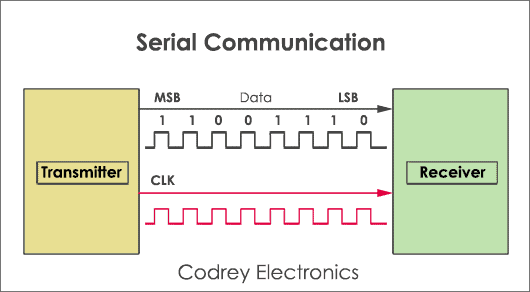
\includegraphics[width=0.5\textwidth]{img/Serial.png}
\caption{Esquema de comunicación serial \cite{serial_communication_basics}.}
\label{fig:serial_communication}
\end{figure}



\subsection{Herramientas Hardware}

\begin{itemize}

\item \textbf{Microcontrolador arduino UNO R3:} (Figura \ref{fig:Arduino})
La placa Arduino UNO R3 está basada en el microcontrolador ATMega328P. Tiene pines para entradas y salidas tanto digitales como analógicas, lo que permite conectarla a varios sensores y dispositivos. Es fácil de programar usando el Arduino IDE y permite cargar programas a través de una conexión USB \cite{ArduinoUNO3}.

\begin{figure}[h]
\centering
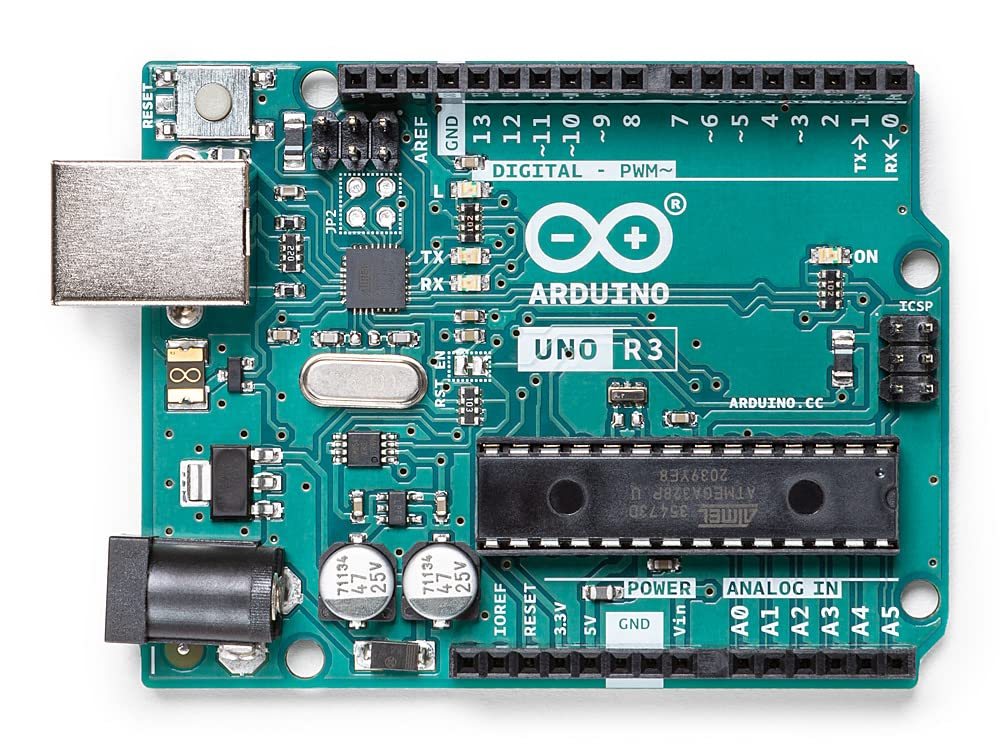
\includegraphics[width=0.5\textwidth]{img/arduinouno.jpg}
\caption{Microcontrolador Arduino UNO R3 \cite{ArduinoUNO3}.}
\label{fig:Arduino}
\end{figure}
\end{itemize}

\begin{itemize}
\item \textbf{Cable USB:} (Figura \ref{fig:usb
})
Conector para cargar el programa en el microcontrolador de Arduino a través del ordenador. Es fundamental para la carga de programas y la comunicación entre la placa y el entorno de desarrollo Arduino IDE. El cable USB también proporciona alimentación a la placa durante la programación y el desarrollo de proyectos. En este caso también tiene la función de enviar los datos recogidos por el sensor a través del puerto COM al que esta conectado y poder visualizarlo en la aplicación de escritorio en tiempo real.


\begin{figure}[h]
\centering
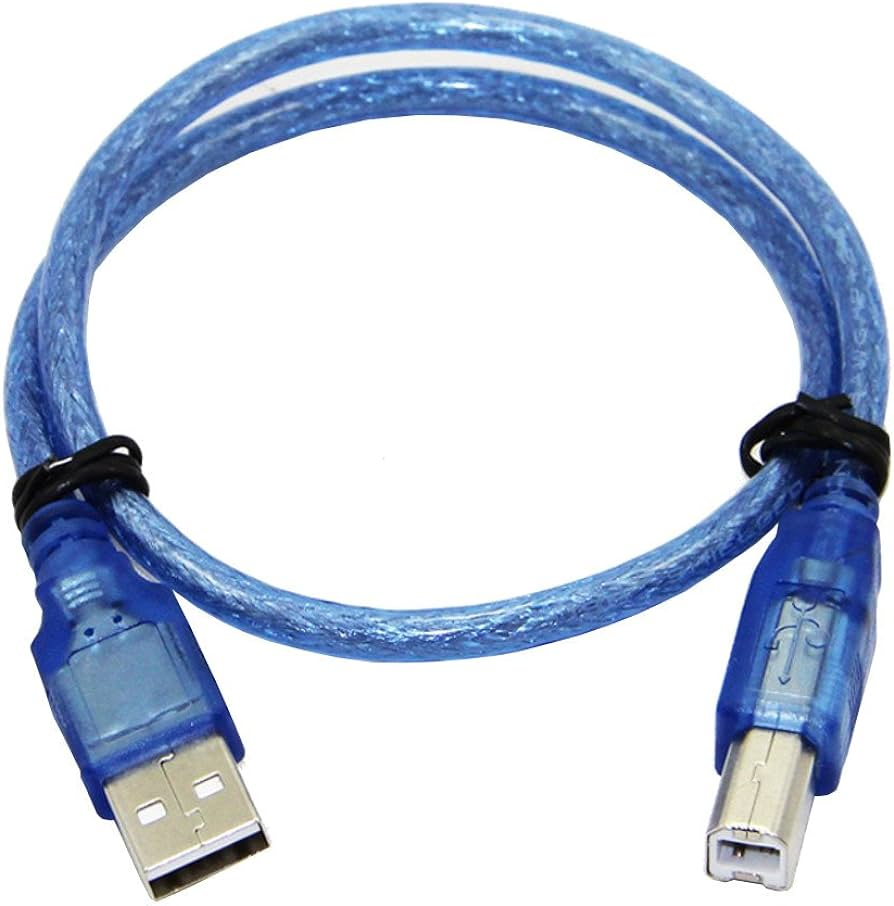
\includegraphics[width=0.5\textwidth]{img/cableUSB.jpg}
\caption{Cable para Conexión USB-Arduino \cite{CableUSB}.}
\label{fig:usb
}
\end{figure}
\end{itemize}


\begin{itemize}
\item \textbf{Cables:} (Figura \ref{fig:Cables
})
Componentes necesarios para conectar el sensor de ECG al Arduino.

\begin{figure}[h]
\centering
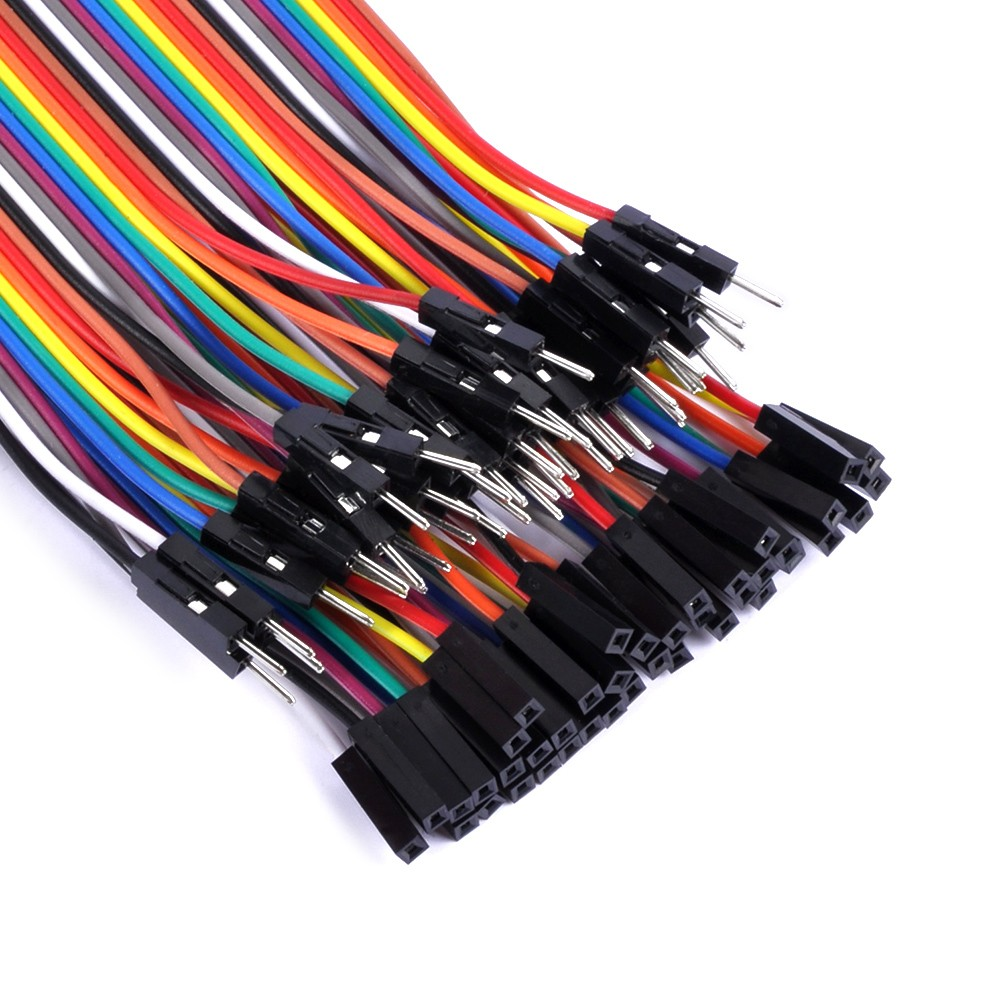
\includegraphics[width=0.5\textwidth]{img/cablesarduino.jpg}
\caption{Cables \cite{Cables}.}
\label{fig:Cables
}
\end{figure}
\end{itemize}

\begin{itemize}
\item \textbf{Electrodos:} (Figura \ref{fig:electrodos})
Componentes necesarios para conectar el sensor de ECG al cuerpo del paciente, asegurando una buena calidad de señal. Estos electrodos son adhesivos y desechables, diseñados para adherirse a la piel del paciente y proporcionar una conexión estable y confiable. La calidad de los electrodos es crucial para obtener lecturas precisas y minimizar el ruido en los datos de ECG. Generalmente están fabricados con materiales conductores que permiten captar las señales eléctricas generadas por el corazón y transmitirlas al sensor de ECG \cite{ElectrodosECG}.

\begin{figure}[h]
\centering
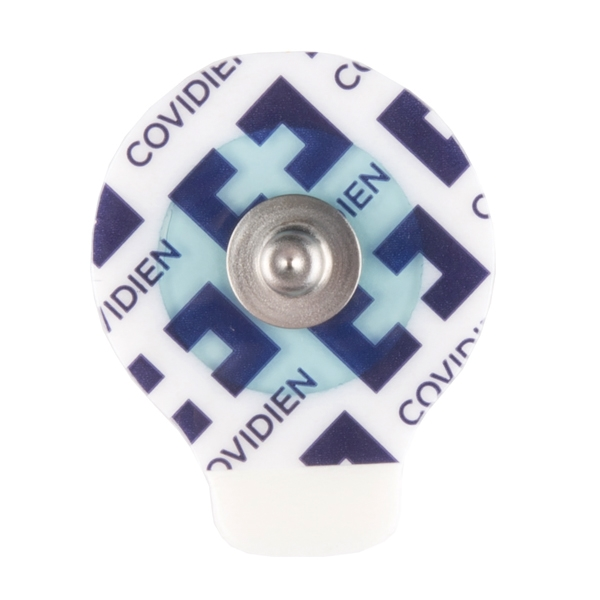
\includegraphics[width=0.5\textwidth]{img/electrodo.jpg}
\caption{Electrodos \cite{ElectrodosECGPediatricos}.}
\label{fig:electrodos}
\end{figure}
\end{itemize}


\subsection{Comparación de diferentes sensores a emplear}

\begin{itemize}
\item \textbf{Módulo AD8232:} (Figura \ref{fig:ad8232})
El módulo AD8232 es un dispositivo que se utiliza para medir señales de ECG y otros biopotenciales. Su función es capturar, aumentar y limpiar las señales eléctricas del cuerpo, incluso en entornos ruidosos. Este módulo facilita que un convertidor analógico-digital (ADC) de bajo consumo o un microcontrolador puedan leer fácilmente la señal de salida \cite{AD8232_teoria}.

\begin{figure}[h]
\centering
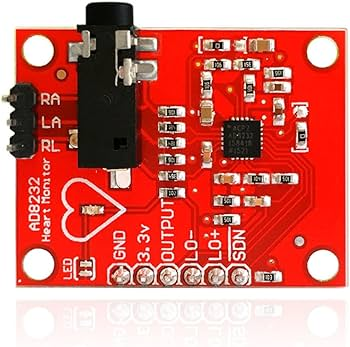
\includegraphics[width=0.5\textwidth]{img/ad8232.jpg}
\caption{Módulo AD8232 \cite{AD8232}.}
\label{fig:ad8232}
\end{figure}

\item \textbf{Sensor KY-039:} (Figura \ref{fig:ky039})
El sensor KY-039 es un módulo de pulso cardíaco que se basa en un emisor y receptor de luz infrarroja para detectar el pulso cardíaco. Funciona al medir la variación en la luz reflejada o absorbida por el flujo sanguíneo en el dedo del usuario. Aunque no es tan preciso como el módulo AD8232 para medir ECG, es una opción más económica y fácil de usar para aplicaciones menos críticas donde se requiere la detección básica del ritmo cardíaco \cite{KY039_teoria}.

\begin{figure}[h]
\centering
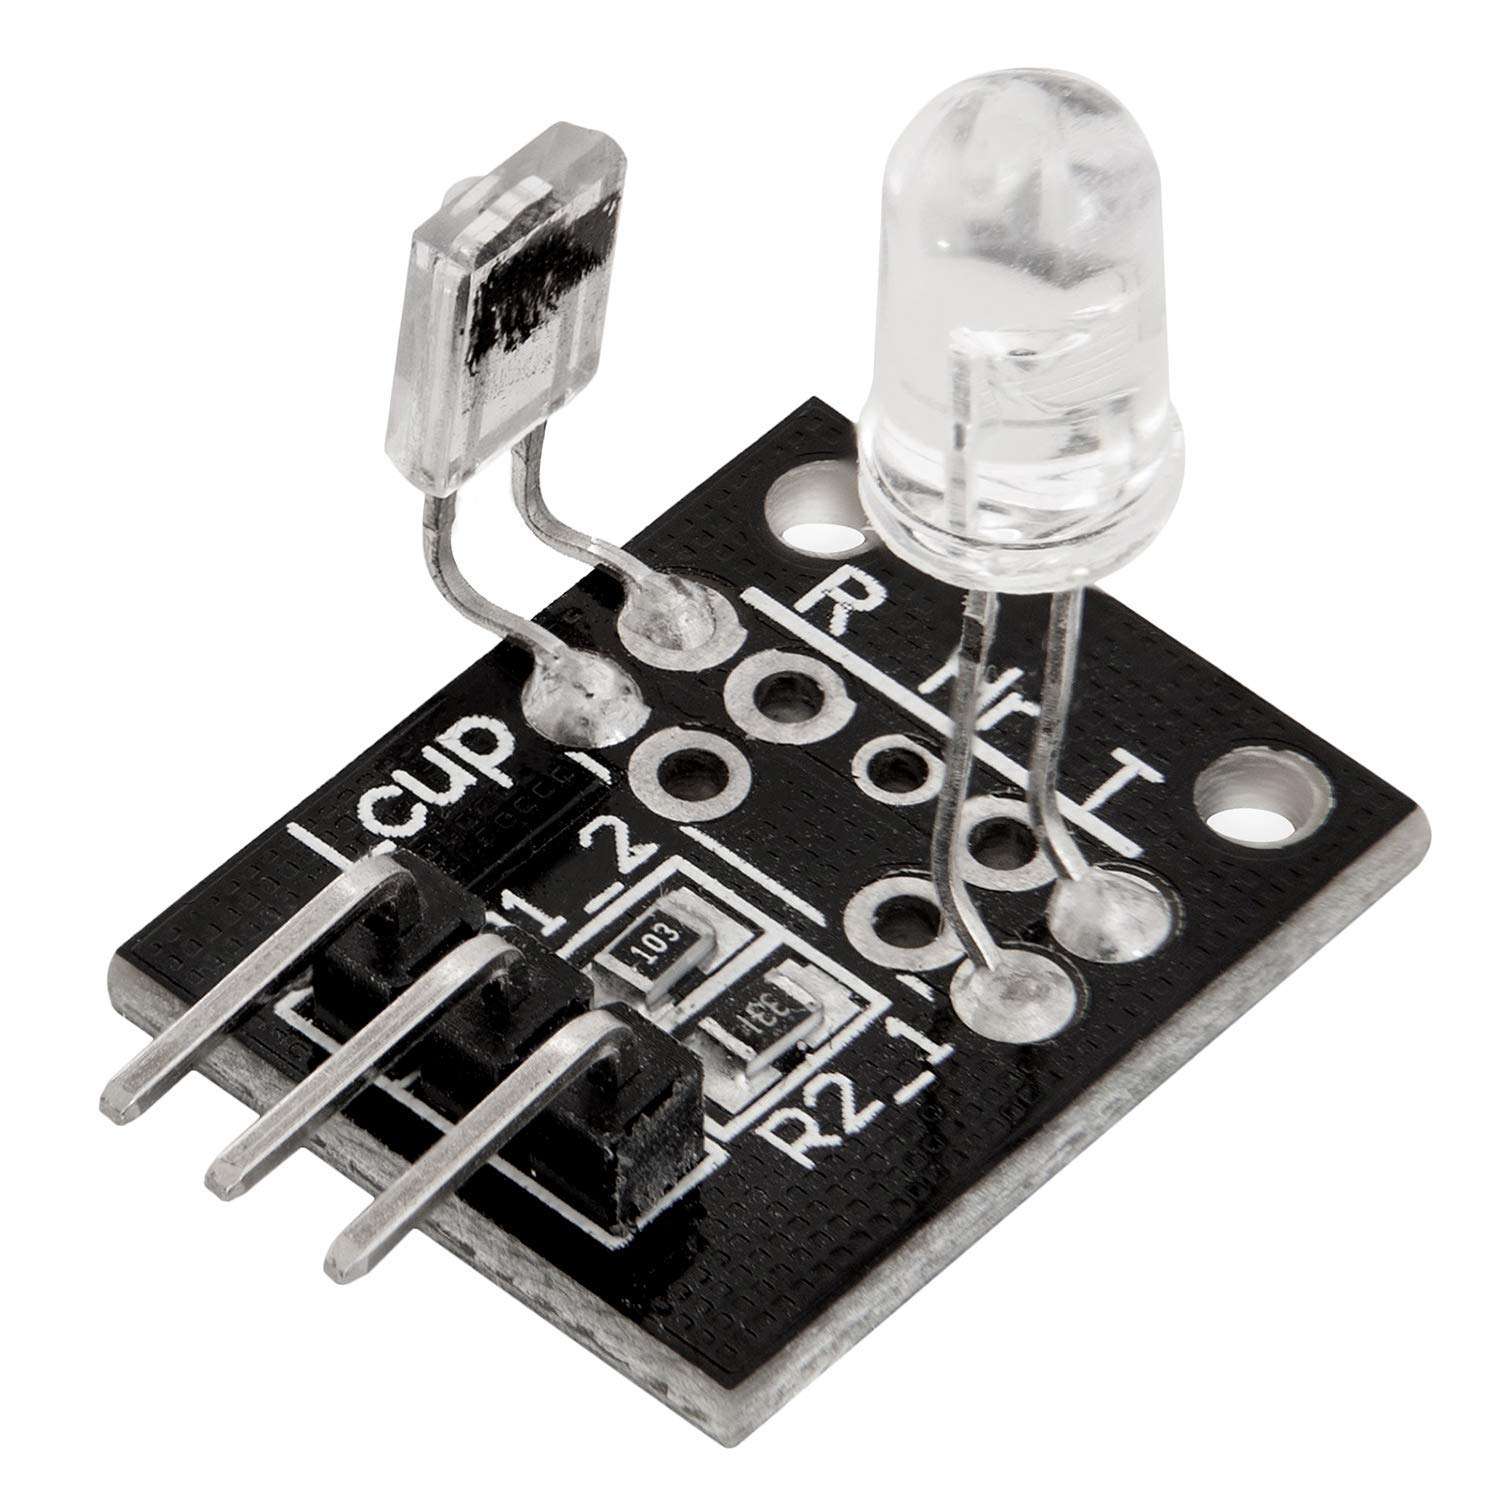
\includegraphics[width=0.5\textwidth]{img/ky-039.jpg}
\caption{Sensor KY-039 \cite{KY039}.}
\label{fig:ky039}
\end{figure}

\item \textbf{Módulo MAX30100:} (Figura \ref{fig:max30100})
El módulo MAX30100 es un sensor de pulso y oxímetro de alta precisión. Combina un pulsioxímetro y un sensor de ritmo cardíaco. Es ideal para aplicaciones que requieren monitoreo de salud a nivel profesional. Necesita una tensión de entrada de 1.8V y es capaz de medir la saturación de oxígeno en sangre junto con la frecuencia cardíaca \cite{MAX30100_teoria}.

\begin{figure}[h]
\centering
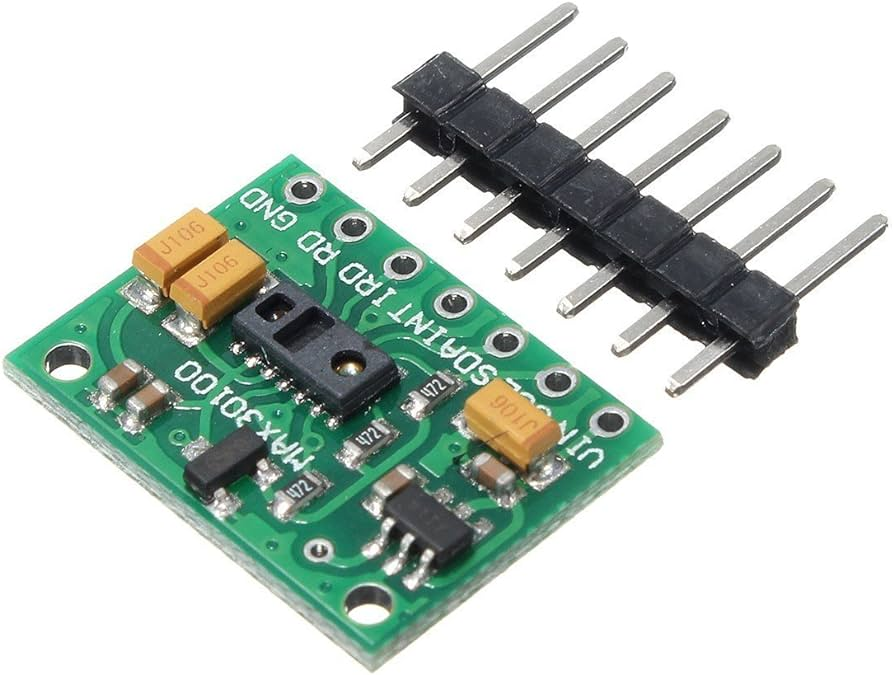
\includegraphics[width=0.5\textwidth]{img/max30100.jpg}
\caption{Módulo MAX30100 \cite{MAX30100}.}
\label{fig:max30100}
\end{figure}

\end{itemize}

\subsection{Conclusión}

En conclusión, he elegido el módulo AD8232 por su alta precisión y capacidad para manejar señales ECG, lo cual es muy importante para tener mediciones fiables y detalladas del ECG. Aunque el sensor KY-039 es más económico y fácil de usar, su precisión es bastante baja y está más orientado a aplicaciones donde solo se necesita la detección del ritmo cardíaco. El módulo MAX30100, aunque ofrece la ventaja de medir la saturación de oxígeno en sangre, es más costoso, por lo que el AD8232 sigue siendo la mejor opción para el balance entre precisión, costo y facilidad de uso en este proyecto.

El AD8232 es capaz de extraer, amplificar y filtrar señales biopotenciales pequeñas, lo que lo hace ideal para nuestro proyecto de monitoreo cardíaco en tiempo real, donde la exactitud y la fiabilidad de los datos son la clave de todo el proyecto. Además, tiene la capacidad de integrarse fácilmente con un microcontrolador. En resumen, aunque el costo del AD8232 es más alto, su precisión y capacidad para operar en condiciones difíciles justifican su elección para el proyecto (ver Tabla \ref{tab:camparacion}).

\begin{table}[h]
	\centering
	\rowcolors{2}{gray!25}{white}
	\begin{tabularx}{\linewidth}{ p{0.3\columnwidth} p{0.4\columnwidth} p{0.2\columnwidth} }
		\toprule
		\textbf{Módulos} & \textbf{Características} & \textbf{Precio} \\
		\toprule
		\textbf{Módulo AD8232} & Mide señales ECG, alta precisión, adecuado para condiciones ruidosas & 10-20€ \\
		\textbf{Sensor KY-039} & Detección básica del ritmo cardíaco mediante luz infrarroja & 3-10€ \\
		\textbf{Módulo MAX30100} & Mide frecuencia cardíaca y saturación de oxígeno en sangre, alta precisión & 15-25€ \\
		\bottomrule
	\end{tabularx}
	\caption{Resumen y comparación de posibles sensores a emplear en el proyecto.}
	\label{tab:camparacion}
\end{table}


\subsection{Mejoras hardware}

He implementado unas pequeñas mejoras en el prototipo para añadir comodidad al paciente y un mejor entendimiento. Se ha añadido un LED que se enciende por cada latido del corazón, lo cual nos puede ayudar a ver que todo está correctamente conectado y en funcionamiento antes de su puesta en marcha en la aplicación web. Además, para una mayor comodidad y orden con los diferentes cables del prototipo, he diseñado una caja para imprimirla en una impresora 3D y que el Arduino y todo el cableado se encuentre en su interior. Hardware empleado para las mejoras:

\begin{itemize}
\item \textbf{Caja en 3D:} (Figura \ref{fig:Caja
})
Esta fabricada con una impresora 3D con material PLA+, tiene como principal función proteger el Arduino, las conexiones entre todos los componentes y sobretodo mantener ordenados los cables que están conectados al Arduino. La caja cuenta con perforaciones diseñadas para:
\begin{itemize}
\item Visualizar del LED.
\item Conexión USB del microprocesador Arduino UNO para cargar los programas y conexión con la aplicación web.
\item Organización de cables para mantener un aspecto ordenado.
\end{itemize}

\begin{figure}[h]
\centering
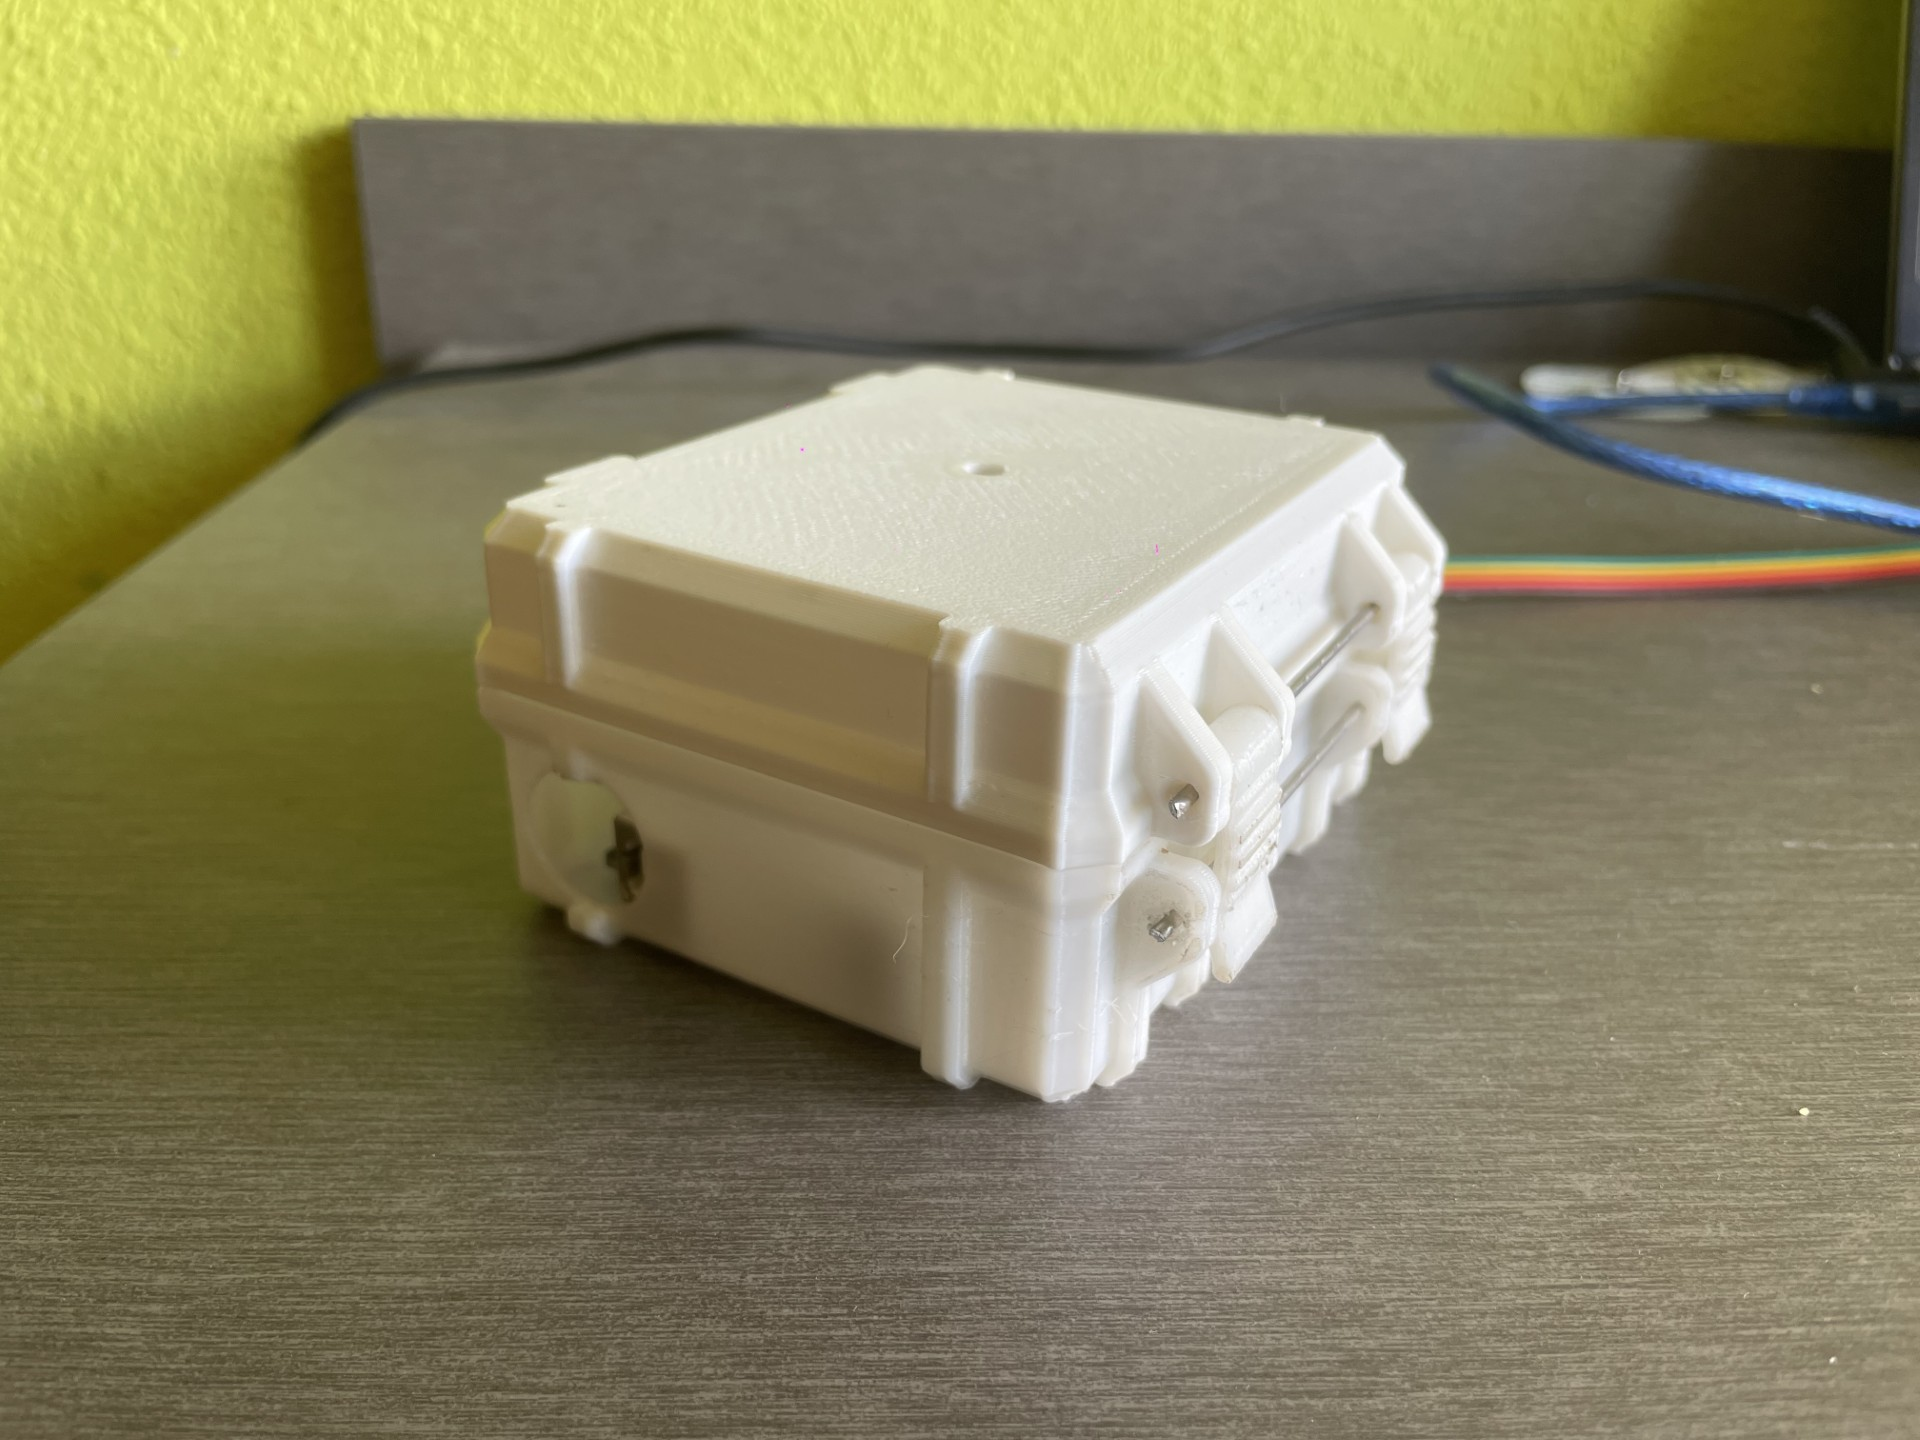
\includegraphics[width=0.5\textwidth]{img/caja3d.jpg}
\caption{Caja para Prototipos fabricada mediante impresión 3D (Fuente propia).}
\label{fig:Caja
}
\end{figure}
\end{itemize}

\begin{itemize}
\item \textbf{LED para Marcar el Pulso del Paciente:} (Figura \ref{fig:LED
})
Conectado al pin 13 (salida digital de Arduino), el LED parpadea en sincronía con el pulso del paciente, proporcionando una indicación visual del ritmo cardíaco y también tiene la función de indicar que todo está funcionando correctamente de cara a realizar la grabación de los datos para su posterior análisis.

\begin{figure}[h]
\centering
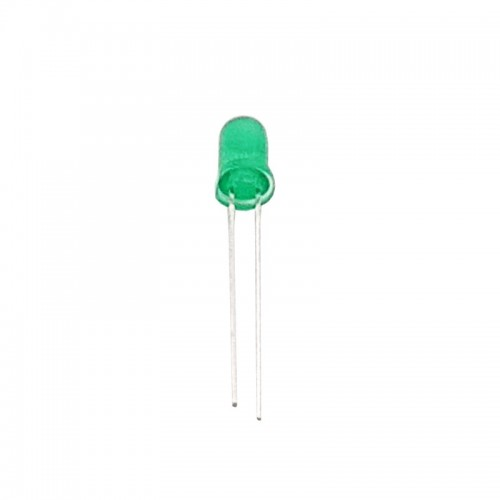
\includegraphics[width=0.5\textwidth]{img/ledverde.jpg}
\caption{LED para Marcar el Pulso del Paciente \cite{LED}.}
\label{fig:LED
}
\end{figure}
\end{itemize}

\begin{itemize}
\item \textbf{Resistencias para el LED:} (Figura \ref{fig:Resistencias
})
Utilizadas para limitar la corriente que pasa a través del LED y otros componentes, protegiendo el circuito de posibles daños. Estas resistencias se calcularon para asegurar un funcionamiento óptimo y seguro.

\begin{figure}[h]
\centering
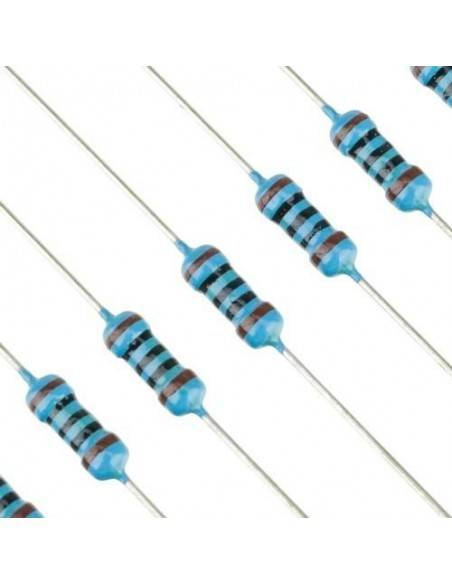
\includegraphics[width=0.5\textwidth]{img/resistencia.jpg}
\caption{Resistencias necesarias para el correcto funcionamiento del circuito \cite{Resistencia}.}
\label{fig:Resistencias
}
\end{figure}
\end{itemize}































